
\section{The Interference of Light}

\makelabheader %(Space for student name, etc., defined in master.tex)

\textbf{Objective}

\begin{itemize}
\item To investigate the interference of light waves as they pass through
a set of slits. 
\end{itemize}
\textbf{Apparatus}

\begin{itemize}
\item Basic optics diode laser
\item Optical bench with rotary motion sensor
\item Phototransistor for measuring light intensity (mounted on rotary motion sensor)
\item ``Multiple Slit Set'' slit accessory
\item Glass plate with sets of narrow slits
\item {\it DataStudio} 750 Interface
\end{itemize}
\textbf{Introduction}

In this laboratory you will investigate the interference of light
produced by a laser beam passing through a set of narrow, adjacent
slits. When light passes the slits each opening acts as an independent
source of waves that can overlap one another to produce a distinctive
pattern of bright and dark spots on a screen. The position of the
bright spots depends on the separation of the adjacent slits and the
wavelength of the incident light. 

You can measure this interference pattern with the setup shown below. 
(This is a \underline{top} view of the set-up.) 
A phototransistor is seated behind the narrow opening on top of the large,
metal mount sitting on a rail. The phototransistor can translate the intensity 
of the light falling on it into a voltage signal that can be read by the
computer. In addition, the phototransistor can be moved back and
forth on a rotary motion sensor that measures the position of the 
mount. These two signals can be combined to
make a graph of the intensity as a function of position.

\vspace{0.3cm}
%{\centering \resizebox*{0.75\textwidth}{!}{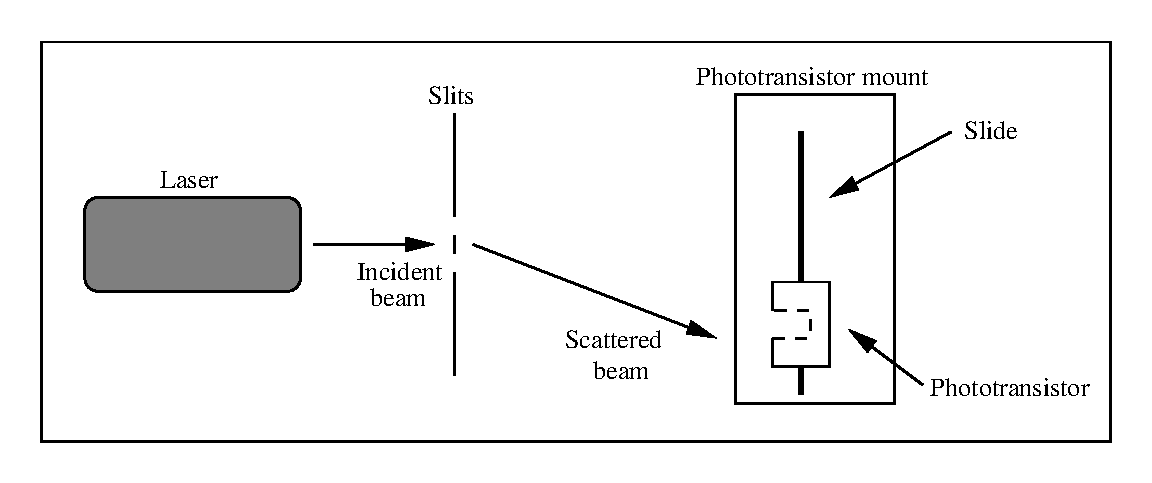
\includegraphics{interference_of_light/interference_of_light_fig_1.eps}} \par}
{\centering \resizebox*{0.75\textwidth}{!}{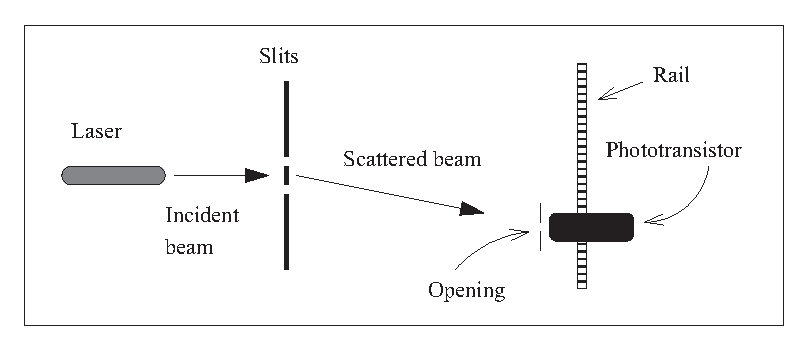
\includegraphics{interference_of_light/interference_of_light_fig1b_bw.eps}} \par}
\vspace{0.3cm}

In this unit you will pass light from the laser through slits of known
separation and use the interference pattern to determine the wavelength
of the light.

\textbf{Activity 1: An Alternative View}

Isaac Newton believed that light was made up of small, unseen particles
that obeyed (surprisingly enough!) Newton's Laws. This view is known
as the corpuscular theory. We want to consider how this model of light
predicts different behavior from the wave theory.

\vspace{35mm}
(a) Consider a laser beam shining on a circular hole. If a beam of
light consisted of small, unseen particles that behaved as tiny billiard
balls what would you see on a screen that is downstream from the circular
hole? A sketch might be useful here.
\vspace{30mm}

(b) Now consider the same laser beam shining on a pair of narrow slits.
What would you see on a screen downstream from the slits if light
were made of corpuscles?
\vspace{30mm}

For the questions above you should have predicted that the laser would
form a single bright spot (for part a) or two parallel lines (for part
b). The experiment you are about to perform provided compelling evidence
that Newton's corpuscular theory was wrong. 

\textbf{Activity 2: The Interference of Light }

(a) You are now ready to turn on the laser. DO NOT LOOK DIRECTLY INTO
THE BEAM OR POINT THE LASER CARELESSLY ABOUT THE ROOM. Mount the laser on the 
optical bench at the opposite end from the rotary motion sensor. Turn on the
laser and you should see the bright red spot of the beam striking
the rotary motion sensor assembly. On the ``Multiple Slit Set'' accessory, 
select a double slit of width .04 mm amd separation .125 mm. Rotate the 
wheel so that the double slit is at the center of the opening.
%You should have a glass plate with a green border and several
%different slit arrangements on it. Place the opening in the center
%of the plate in the path of the laser beam. The adjacent slits in
%the center hole are 0.03295 mm apart. What do you see? 
\vspace{10mm}

%(b) Position the glass plate about 30-40 cm from the phototransistor
%mount with the central maximum (the brightest spot) 
%striking the center hole. Measure and record this
%distance. You may find it useful to use the plumb line to measure
%this distance.
(b) Position the double slit about 70 cm from the phototransistor mount. Adjust 
the laser beam direction so that it falls on the double slit you have selected. 
(There are two adjustment screws on the back of the laser.) 
You should see the interference pattern on the phototransistor mount. 
\vspace{10mm}

(c) Position the phototransistor mount so the interference pattern
is at the same height as the opening in the center of the phototransistor mount. The phototransistor is mounted behind this hole. To make accurate measurements it is important to carefully determine the geometry of your setup. Check to see if the slits and the phototransistor mount are perpendicular to the incident
laser beam.  You want to make sure the phototransistor can {}``see'' as many
bright spots as possible. Carefully slide the phototransistor mount back and forth to make sure that it stays centered on the interference pattern. Then set it 
at one side of the pattern to begin the experiment.
Start the ``Interference'' activity in the {\bf 132 Workshop} folder. 
When you are ready, click {\bf Start} and slowly move the phototransistor 
from one side of the slide to the other by turning the wheel on the rotary 
motion sensor. Move carefully and take about 4-5 seconds to complete the 
motion. Click {\bf Stop}.
When data acquisition is complete you will see a graph representing
the intensity reading versus the position reading. You should see
several distinct peaks. This graph is the interference pattern. If
you do not see this pattern consult your instructor. Add the title ``Double 
Slit Interference/Diffraction Pattern'' and the axis labels ``Relative 
Intensity'' (vertical) and ``Position (m)'' (horizontal). Make a hardcopy
of this graph and attach it to this unit.

\newpage

(d) In theory, the interference pattern should look like the figure at the 
bottom of page 915 of your textbook (also shown in Fig. 2 of the next 
experiment). The intensity is just a $cos^2$ function. Obviously, the pattern 
doesn't look like that. The reason is that light from each slit undergoes 
single slit diffraction which we will study in the next experiment. (That's 
why we are calling the pattern an ``inteference/diffraction'' pattern.) 
But the peaks should still be equally spaced. 
Is the spacing between the intensity peaks constant? Is the intensity
of each peak the same? Does it appear that any peaks are missing?
The more peaks you see the more (and hopefully better) data you can collect.
There is a button on top of the phototransistor labeled ``Gain'' which changes
the size of the intensity signal. Try changing this setting to see if you can 
get more peaks in your spectrum (do this only if necessary).
\vspace{15mm}

(e) Now switch to 3 slits by rotating the wheel on the slit accessory 
appropriately, and run the pattern again. You will see that the peaks are 
narrower, because the pattern is not just a $cos^2$ function; it is more 
complicated. Now try 4 slits and then 5 slits. In each case the peaks are a bit 
narrower, although overall the pattern is similar because you haven't changed 
the slit width or the slit separation. 

(f) Now switch to the center opening in the glass plate. This has 15 or 20 
slits, so the peaks will be narrower still. In this case the the slit 
separation is 0.03295 mm, so the maxima will be farther apart than in the 
previous cases. Run the pattern again. Measure the distance from the glass plate
 to the phototransistor as accurately as possible (the distance $L$ below), 
realizing that the phototransistor lies 25.4 mm behind the opening in the mount.

(g) When you are satisfied with the quality of your spectrum record the 
position of each peak in the left column of the table below, with the central 
peak halfway down the column. Use the {\bf Smart Tool} to accurately read off 
the peak positions by clicking on the appropriate button along the top of the 
graph. A set of cross-hairs will appear on the plot. Grab the cross-hairs by 
clicking on them and dragging them to the point you want to measure.
The coordinates will be printed by the cross-hairs.
Turn off the laser when you are finished. Print the graph with the title 
``Multiple slit Interference/Diffraction pattern'' and the same axis labels as 
before.

\vspace{0.3cm}
{\centering \begin{tabular}{|c|c|}
\hline 
Position Reading (m)&
Change in Reading (m)\\
\hline
\hline 
&
\\
\hline 
&
\\
\hline 
&
\\
\hline 
&
\\
\hline 
&
\\
\hline 
&
\\
\hline 
&
\\
\hline
&
\\
\hline
&
\\
\hline
&
\\
\hline
&
\\
\hline
\end{tabular}\par}
\vspace{0.3cm}

\textbf{Activity 3: Determining the Wavelength of the Laser }

(a) For the data you recorded in the previous activity, calculate the 
difference between each pair of adjacent readings and record it in the 
right column of the above table (first space will be blank).

(b) Calculate the average and standard deviation of the separation between 
adjacent peaks (right hand column values). Don't forget units.
\vspace{15mm}

\newpage

(c) The position of the interference maxima can be described by (see text p. 
914)

\[
y_{m}=\frac{\lambda L}{d}m\]


where $y_{m}$ is the distance of a bright spot from the central
maximum (the distance along the slide in this experiment) and $L$ is
the distance from the slits to the phototransistor. The quantity $d$
is the slit separation, \( \lambda  \) is the wavelength of the light,
and $m$ is the order of the bright spot. Generate an expression for
the distance $\Delta y$ between adjacent bright spots.
\vspace{20mm}

(d) Use the expression you generated in part (c) and the average separation
between bright spots you determined in part (b) to calculate the wavelength of 
the laser light and its uncertainty (both in nm). Show how you get the result 
in nanometers. Compare your result with the wavelength range indicated on the 
laser.
\vspace{40mm}

(e) Collect the results for the wavelength from the other teams in class
and calculate the average and standard deviation. Record the results here. 
(Don't forget units.)
Are your results consistent with the class results? Why or why not?
\vspace{60mm}

(f) Recall the earlier discussion of Newton's corpuscular theory of
light. Does your data support Newton's theory or the wave theory?
Why?\vspace{15mm}

